\chapter{Antecedentes}
\textit{El presente trabajo presenta la construcción de un electrocardiograma convencional utilizando conocimientos de programación en PIC's y adaptando una interfaz en un teléfono con sistema operativo android.}\newline
\textit{Los elementos que vamos a utilizar son:}
\begin{itemize}
\item \textit{Baterias 12V}
\item \textit{Regulador de tension LM317T}
\item \textit{TTL 74LS04}
\item \textit{PIC18F4550}
\item \textit{Electrodos}
\item \textit{Cables para electrocardiografía}
\item \textit{Adaptadores para cables electrocardiógrafos}
\end{itemize}
Así como se puede consultar en el trabajo recepcional de tesis de Guillermo Eduardo Vega Picón

\begin{figure}
   	\centering
		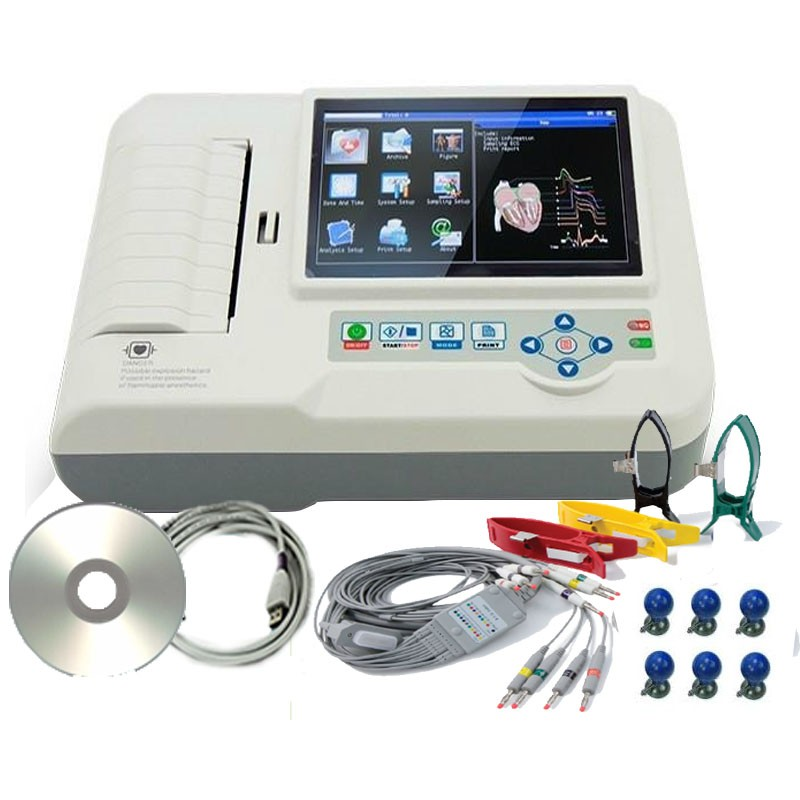
\includegraphics[width=12cm]{imag/electrocardiografo.jpg}
		\caption{Electrocardiografo.}
		\label{cavi}
\end{figure}